\scanpage{66}
% archive sheet number: 65
% The entire draft is cancelled by a long diagonal stroke; two additional nearly vertical cancellation strokes flank the proof.
\deleted{This gives a more pleasant and elementary proof of 11.9.6. As for 11.9.3. (ii), it will follow from a}

\deleted{\uline{Lemma} (or cor\rlap{l}ollary to the preceding proposition). Under the hypotheses of the proposition, let us no longer necessarily assume that $A'$ is projective over $A$, but only this: for every integral domain quotient $B=A/\underline{p}$ of $A$, setting $B'=B\otimes_A A'$, there exists an $h\quad B-(0)$ such that $B_h$ is \mbox{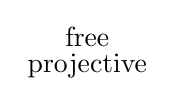
\begin{tikzpicture}[baseline=(base.base)]
\node[inner sep=0] (base) {\deleted{projective}};
\node[anchor=south,inner sep=0,yshift=.08cm] at (base.north) {\inserted{free}};
\end{tikzpicture}} over $A_h$. Then the conclusion of the proposition still remains valid.}

\deleted{Indeed, let $\handwritten{\phi}$ be a section of $F'$ whose images under the $u'$ are zero, let us prove $\handwritten{\phi}=0$, i.e. $\operatorname{supp}\handwritten{\phi}=\handwritten{\unsure{\varnothing|\phi}}$. Otherwise, there would exist a maximal point $x'$ in $\operatorname{supp}\handwritten{\phi}$, corresponding to the prime ideal $\underline{p}'$ of $A'$. Let \mbox{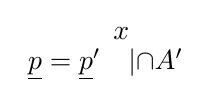
\begin{tikzpicture}[baseline=(base.base)]
\node[inner sep=0] (base) {$\deleted{\underline{p}=\underline{p}'\unsure{\quad|\cap}A'}$};
\path (base.north west) -- coordinate[pos=.60] (ins) (base.north east);
\node[anchor=south,inner sep=0,yshift=.10cm] at (ins) {\inserted{$x$}};
\end{tikzpicture}} be its image in $X$, defined by the ideal $\underline{p}$, the contraction of $\underline{p}'$ to $A$, then by virtue of the hypothesis applied to $A/\underline{p}$, we see that, up to replacing $X$ by an affine open neighbourhood of $x$, we may assume that $\rlap{\(B\)}A'/\underline{p}\rlap{\(B\)}A'$ is \mbox{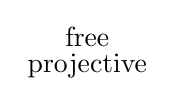
\begin{tikzpicture}[baseline=(base.base)]
\node[inner sep=0] (base) {\deleted{projective}};
\node[anchor=south,inner sep=0,yshift=.08cm] at (base.north) {\inserted{free}};
\end{tikzpicture}} over $A/\underline{p}$. Note that we could choose $x'$ in such a way that $x$ is also maximal in $g(\operatorname{supp}\handwritten{\phi})$ (start by choosing $x$ maximal in $g(\operatorname{supp}\handwritten{\phi})$, then $x'$ maximal in $g^{-1}(x)$), which means that localizing at $\underline{p}$, the support of $\handwritten{\phi}_{\underline{p}}$ is contained in $\operatorname{Spec}(A'_{\underline{p}}/\underline{p}A'_{\underline{p}})$, hence $\handwritten{\phi}_{\underline{p}}$ is annihilated by a power of $\underline{p}\ A'_{\underline{p}}$, or again that we can find $\unsure{\rlap{\(u\)}h|h}\quad A-\underline{p}$ such that}
